\subsection{Comparison of the encoders}
\label{sec:codificadores}

On the test set, the \num{11} encoders lie between \num{25.95} and \qty{28.83}{\cm} in mean 3-D error, a spread of \qty{2.89}{\cm}, with a mean MAE of \num{12.63} to \qty{14.14}{\cm} and a combined RMSE of \num{18.55} to \qty{20.64}{\cm} (Table~\ref{tab:codificadores}). The first four, GATv2-cascade (\qty{25.95}{\cm}), GPS-cascade (\qty{26.06}{\cm}), GATv2 (\qty{26.08}{\cm}) and GPS (\qty{26.27}{\cm}), differ by up to \qty{0.32}{\cm}.

\begin{table}[H]
  \centering
  \caption{The \num{11} encoders of the final comparison, with capacity matched to \num{1843395} parameters, in increasing order of mean 3-D error on the \num{937} test events; mean MAE, combined RMSE and mean 3-D error in cm. $D$: width of the node states; $B$: batch size chosen by the memory probe (\num{128}, \num{256} or \num{512} mirrored training rows, which correspond to \num{22250}, \num{11150} and \num{5600} optimisation steps over \num{50} epochs, respectively), with the learning rates multiplied by $B$/\num{128}. $^{\dagger}$: does not read the edge features. The first four cannot be distinguished by the paired resampling (Figure~\ref{fig:diferenca_pareada}).}
  \label{tab:codificadores}
  \begin{tabular}{@{}l S[table-format=3.0] S[table-format=1.3] S[table-format=3.0] S[table-format=2.2] S[table-format=2.2] S[table-format=2.2]@{}}
\toprule
 & {} & {Parameters} & {} & {Mean} & {RMSE} & {Mean 3-D} \\
Encoder & {$D$} & {(\num{e6})} & {$B$} & {MAE (cm)} & {comb.\ (cm)} & {error (cm)} \\
\midrule
GATv2-cascade & 212 & 1.869 & 128 & 12.63 & 18.64 & 25.95 \\
GPS-cascade & 132 & 1.874 & 128 & 12.79 & 18.69 & 26.06 \\
GATv2 & 204 & 1.819 & 128 & 12.74 & 18.80 & 26.08 \\
GPS & 128 & 1.843 & 256 & 12.95 & 18.55 & 26.27 \\
GeneralConv & 280 & 1.833 & 256 & 12.86 & 18.94 & 26.43 \\
ResGatedGCN$^{\dagger}$ & 292 & 1.841 & 512 & 13.07 & 19.02 & 26.71 \\
GraphSAGE$^{\dagger}$ & 400 & 1.840 & 512 & 13.23 & 19.01 & 26.92 \\
EdgeConv$^{\dagger}$ & 685 & 1.843 & 128 & 13.46 & 20.23 & 27.67 \\
PNA & 147 & 1.841 & 512 & 13.52 & 19.57 & 27.68 \\
GINE & 395 & 1.844 & 512 & 13.81 & 20.21 & 28.23 \\
GINE-cascade & 404 & 1.843 & 512 & 14.14 & 20.64 & 28.83 \\
\bottomrule
\end{tabular}

\end{table}

The paired differences in mean 3-D error relative to GATv2-cascade are \qty[retain-explicit-plus]{+0.12}{\cm} (\num{-0.30} to \qty{0.54}{\cm}) for GPS-cascade, \qty[retain-explicit-plus]{+0.13}{\cm} (\num{-0.28} to \qty{0.55}{\cm}) for GATv2 and \qty[retain-explicit-plus]{+0.32}{\cm} (\num{-0.12} to \qty{0.77}{\cm}) for GPS, intervals that contain zero; from GeneralConv onwards (\qty[retain-explicit-plus]{+0.48}{\cm}; \num{0.02} to \qty{0.95}{\cm}), the intervals lie above zero, without correction for multiple comparisons (Figure~\ref{fig:diferenca_pareada}). GATv2-cascade has the lowest mean 3-D error in \qty{56.9}{\percent} of the resamples; GPS, with the lowest combined RMSE (\qty{18.55}{\cm}), leads that metric in \qty{61.8}{\percent} of them; GATv2 has the lowest validation error (\qty{25.72}{\cm}). There is, therefore, no established best encoder. From here on, GATv2-cascade represents the group of the four best; it was chosen by the test metric, a choice that favours its test error, and was trained once, like the others.

Early stopping (\num{15} epochs without improvement on validation) was not triggered; the lowest validation error occurred between epochs \num{41} and \num{50}, in the last epoch for GraphSAGE and GeneralConv. For GATv2-cascade (Figure~\ref{fig:curvas_validacao}), the training error on the mirrored rows ends at \qty{21.91}{\cm}, and the validation and test errors agree (\num{25.96} and \qty{25.95}{\cm}).

\begin{figure}[H]
  \centering
  \begin{subfigure}[t]{0.485\textwidth}
    \centering
    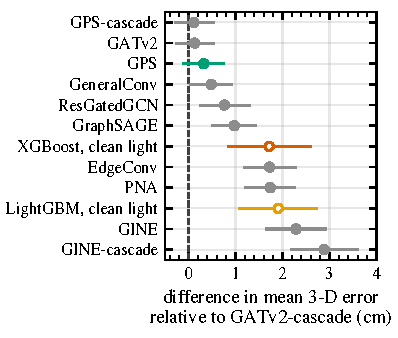
\includegraphics{figures/diferenca_pareada.pdf}
    \caption{Difference in mean 3-D test error relative to that of GATv2-cascade, with a \qty{95}{\percent} interval from paired bootstrap resampling of the \num{937} test events (\num{10000} resamples); GPS, with the lowest combined RMSE, in green; \mbox{XGBoost} and \mbox{LightGBM} on clean light, with hollow markers. Positive differences indicate a higher error than that of GATv2-cascade; the intervals of GPS-cascade, GATv2 and GPS contain zero.}
    \label{fig:diferenca_pareada}
  \end{subfigure}\hfill
  \begin{subfigure}[t]{0.485\textwidth}
    \centering
    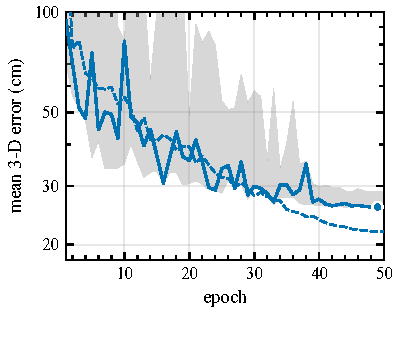
\includegraphics{figures/curvas_validacao.pdf}
    \caption{Mean 3-D error per epoch, on a logarithmic scale: shaded band between the lowest and the highest validation error of the \num{11} encoders and, for GATv2-cascade, the validation curve (solid) and the training curve on the mirrored rows (dashed), with a marker at the epoch of lowest validation error. The training value of the first epoch and the upper edge of the band at several epochs of the first half of training lie above the scale.}
    \label{fig:curvas_validacao}
  \end{subfigure}
  \caption{Comparison of the \num{11} matched-capacity encoders: (a) differences on the \num{937} test events; (b) training curves.}
  \label{fig:par_codificadores}
\end{figure}

The three encoders that do not read the edge features sit in the middle of Table~\ref{tab:codificadores}: ResGatedGCN sixth, GraphSAGE seventh and EdgeConv eighth. The five trained with batch size \num{512} (\num{5600} steps) occupy positions 6, 7, 9, 10 and 11, and the first three used batch size \num{128} (\num{22250} steps): the comparison equalises the number of parameters but does not separate the effect of the operator from that of the optimisation budget.
